% Created by tikzDevice version 0.12.3 on 2019-12-30 23:10:14
% !TEX encoding = UTF-8 Unicode
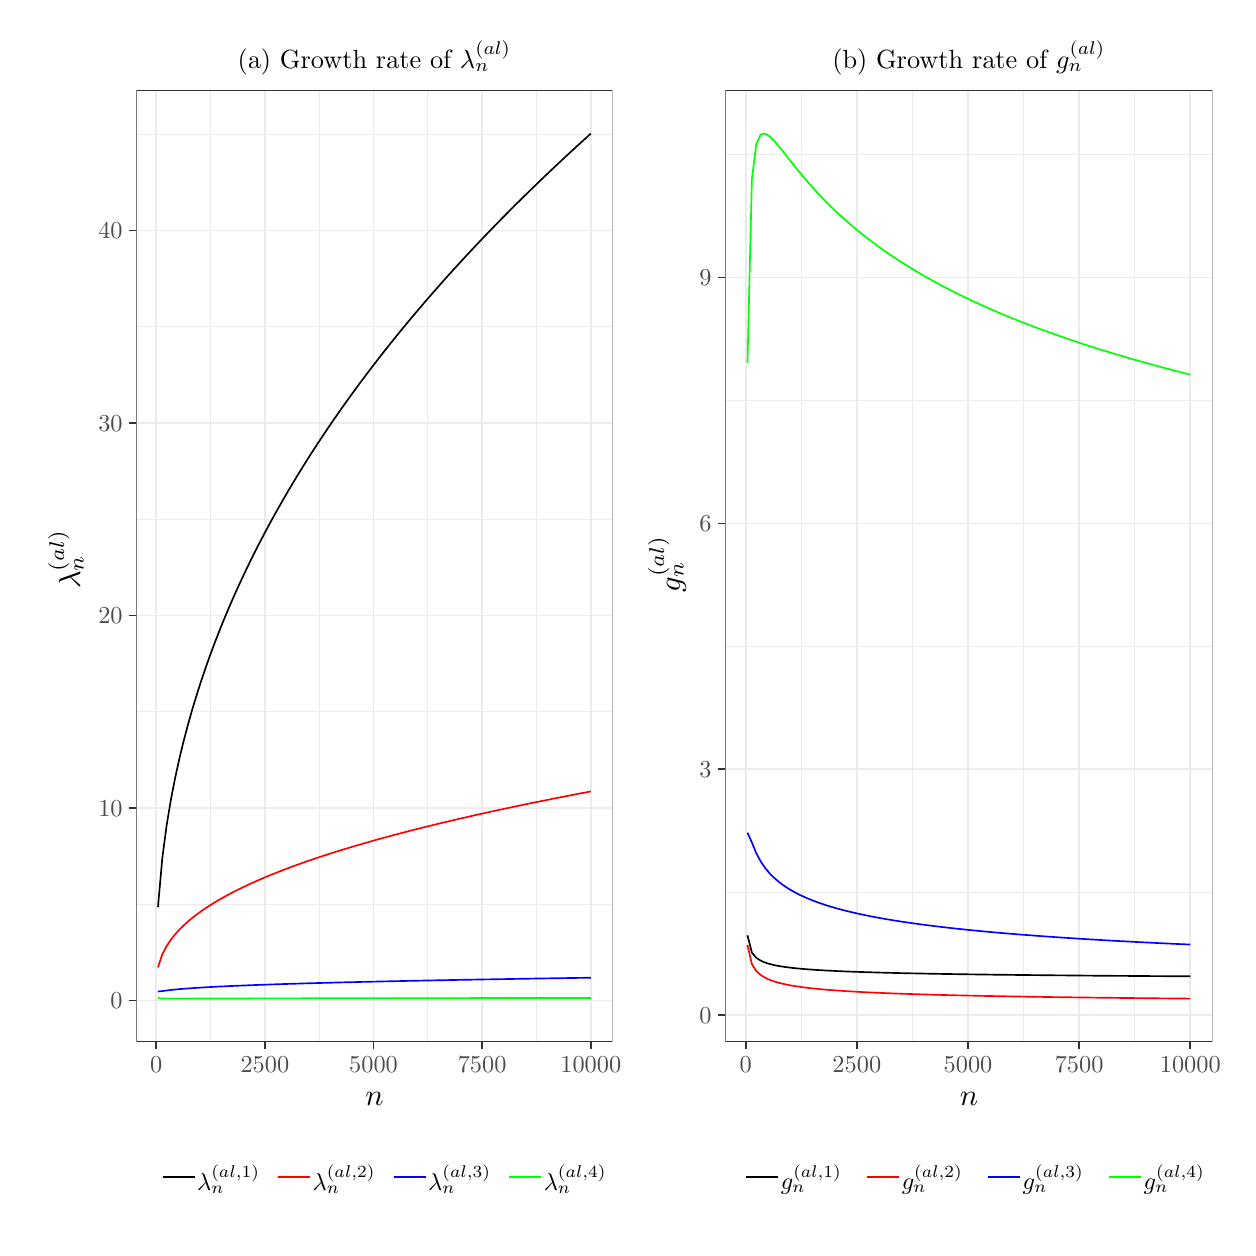
\begin{tikzpicture}[x=1pt,y=1pt]
\definecolor{fillColor}{RGB}{255,255,255}
\path[use as bounding box,fill=fillColor,fill opacity=0.00] (0,0) rectangle (433.62,433.62);
\begin{scope}
\path[clip] (  0.00,  0.00) rectangle (216.81,433.62);
\definecolor{drawColor}{RGB}{255,255,255}
\definecolor{fillColor}{RGB}{255,255,255}

\path[draw=drawColor,line width= 0.6pt,line join=round,line cap=round,fill=fillColor] (  0.00,  0.00) rectangle (216.81,433.62);
\end{scope}
\begin{scope}
\path[clip] ( 39.26, 67.14) rectangle (211.31,410.96);
\definecolor{fillColor}{RGB}{255,255,255}

\path[fill=fillColor] ( 39.26, 67.14) rectangle (211.31,410.96);
\definecolor{drawColor}{gray}{0.92}

\path[draw=drawColor,line width= 0.3pt,line join=round] ( 39.26,116.89) --
	(211.31,116.89);

\path[draw=drawColor,line width= 0.3pt,line join=round] ( 39.26,186.44) --
	(211.31,186.44);

\path[draw=drawColor,line width= 0.3pt,line join=round] ( 39.26,255.98) --
	(211.31,255.98);

\path[draw=drawColor,line width= 0.3pt,line join=round] ( 39.26,325.52) --
	(211.31,325.52);

\path[draw=drawColor,line width= 0.3pt,line join=round] ( 39.26,395.07) --
	(211.31,395.07);

\path[draw=drawColor,line width= 0.3pt,line join=round] ( 66.08, 67.14) --
	( 66.08,410.96);

\path[draw=drawColor,line width= 0.3pt,line join=round] (105.34, 67.14) --
	(105.34,410.96);

\path[draw=drawColor,line width= 0.3pt,line join=round] (144.60, 67.14) --
	(144.60,410.96);

\path[draw=drawColor,line width= 0.3pt,line join=round] (183.86, 67.14) --
	(183.86,410.96);

\path[draw=drawColor,line width= 0.6pt,line join=round] ( 39.26, 82.12) --
	(211.31, 82.12);

\path[draw=drawColor,line width= 0.6pt,line join=round] ( 39.26,151.66) --
	(211.31,151.66);

\path[draw=drawColor,line width= 0.6pt,line join=round] ( 39.26,221.21) --
	(211.31,221.21);

\path[draw=drawColor,line width= 0.6pt,line join=round] ( 39.26,290.75) --
	(211.31,290.75);

\path[draw=drawColor,line width= 0.6pt,line join=round] ( 39.26,360.30) --
	(211.31,360.30);

\path[draw=drawColor,line width= 0.6pt,line join=round] ( 46.45, 67.14) --
	( 46.45,410.96);

\path[draw=drawColor,line width= 0.6pt,line join=round] ( 85.71, 67.14) --
	( 85.71,410.96);

\path[draw=drawColor,line width= 0.6pt,line join=round] (124.97, 67.14) --
	(124.97,410.96);

\path[draw=drawColor,line width= 0.6pt,line join=round] (164.23, 67.14) --
	(164.23,410.96);

\path[draw=drawColor,line width= 0.6pt,line join=round] (203.49, 67.14) --
	(203.49,410.96);
\definecolor{drawColor}{RGB}{0,0,0}

\path[draw=drawColor,line width= 0.6pt,line join=round] ( 47.08,115.82) --
	( 48.65,133.57) --
	( 50.21,145.37) --
	( 51.77,154.76) --
	( 53.34,162.77) --
	( 54.90,169.85) --
	( 56.47,176.26) --
	( 58.03,182.16) --
	( 59.59,187.64) --
	( 61.16,192.78) --
	( 62.72,197.64) --
	( 64.29,202.25) --
	( 65.85,206.65) --
	( 67.41,210.86) --
	( 68.98,214.91) --
	( 70.54,218.81) --
	( 72.11,222.57) --
	( 73.67,226.22) --
	( 75.23,229.75) --
	( 76.80,233.18) --
	( 78.36,236.52) --
	( 79.93,239.77) --
	( 81.49,242.95) --
	( 83.05,246.04) --
	( 84.62,249.07) --
	( 86.18,252.03) --
	( 87.75,254.93) --
	( 89.31,257.77) --
	( 90.88,260.56) --
	( 92.44,263.29) --
	( 94.00,265.98) --
	( 95.57,268.62) --
	( 97.13,271.21) --
	( 98.70,273.76) --
	(100.26,276.27) --
	(101.82,278.74) --
	(103.39,281.18) --
	(104.95,283.58) --
	(106.52,285.94) --
	(108.08,288.28) --
	(109.64,290.58) --
	(111.21,292.85) --
	(112.77,295.09) --
	(114.34,297.31) --
	(115.90,299.49) --
	(117.46,301.65) --
	(119.03,303.79) --
	(120.59,305.90) --
	(122.16,307.99) --
	(123.72,310.05) --
	(125.29,312.09) --
	(126.85,314.12) --
	(128.41,316.12) --
	(129.98,318.09) --
	(131.54,320.05) --
	(133.11,322.00) --
	(134.67,323.92) --
	(136.23,325.82) --
	(137.80,327.71) --
	(139.36,329.58) --
	(140.93,331.43) --
	(142.49,333.27) --
	(144.05,335.09) --
	(145.62,336.89) --
	(147.18,338.68) --
	(148.75,340.46) --
	(150.31,342.22) --
	(151.87,343.97) --
	(153.44,345.70) --
	(155.00,347.42) --
	(156.57,349.12) --
	(158.13,350.82) --
	(159.70,352.50) --
	(161.26,354.17) --
	(162.82,355.82) --
	(164.39,357.47) --
	(165.95,359.10) --
	(167.52,360.72) --
	(169.08,362.34) --
	(170.64,363.93) --
	(172.21,365.52) --
	(173.77,367.10) --
	(175.34,368.67) --
	(176.90,370.23) --
	(178.46,371.78) --
	(180.03,373.32) --
	(181.59,374.85) --
	(183.16,376.36) --
	(184.72,377.88) --
	(186.28,379.38) --
	(187.85,380.87) --
	(189.41,382.35) --
	(190.98,383.83) --
	(192.54,385.29) --
	(194.11,386.75) --
	(195.67,388.20) --
	(197.23,389.64) --
	(198.80,391.08) --
	(200.36,392.50) --
	(201.93,393.92) --
	(203.49,395.33);
\definecolor{drawColor}{RGB}{255,0,0}

\path[draw=drawColor,line width= 0.6pt,line join=round] ( 47.08, 94.04) --
	( 48.65, 98.76) --
	( 50.21,101.76) --
	( 51.77,104.09) --
	( 53.34,106.06) --
	( 54.90,107.77) --
	( 56.47,109.31) --
	( 58.03,110.72) --
	( 59.59,112.01) --
	( 61.16,113.22) --
	( 62.72,114.36) --
	( 64.29,115.43) --
	( 65.85,116.45) --
	( 67.41,117.43) --
	( 68.98,118.36) --
	( 70.54,119.25) --
	( 72.11,120.11) --
	( 73.67,120.94) --
	( 75.23,121.75) --
	( 76.80,122.52) --
	( 78.36,123.28) --
	( 79.93,124.01) --
	( 81.49,124.73) --
	( 83.05,125.42) --
	( 84.62,126.10) --
	( 86.18,126.76) --
	( 87.75,127.41) --
	( 89.31,128.04) --
	( 90.88,128.66) --
	( 92.44,129.27) --
	( 94.00,129.86) --
	( 95.57,130.45) --
	( 97.13,131.02) --
	( 98.70,131.58) --
	(100.26,132.14) --
	(101.82,132.68) --
	(103.39,133.21) --
	(104.95,133.74) --
	(106.52,134.26) --
	(108.08,134.77) --
	(109.64,135.27) --
	(111.21,135.77) --
	(112.77,136.26) --
	(114.34,136.74) --
	(115.90,137.21) --
	(117.46,137.68) --
	(119.03,138.15) --
	(120.59,138.60) --
	(122.16,139.06) --
	(123.72,139.50) --
	(125.29,139.95) --
	(126.85,140.38) --
	(128.41,140.81) --
	(129.98,141.24) --
	(131.54,141.66) --
	(133.11,142.08) --
	(134.67,142.49) --
	(136.23,142.90) --
	(137.80,143.31) --
	(139.36,143.71) --
	(140.93,144.11) --
	(142.49,144.50) --
	(144.05,144.89) --
	(145.62,145.27) --
	(147.18,145.66) --
	(148.75,146.04) --
	(150.31,146.41) --
	(151.87,146.78) --
	(153.44,147.15) --
	(155.00,147.52) --
	(156.57,147.88) --
	(158.13,148.24) --
	(159.70,148.60) --
	(161.26,148.95) --
	(162.82,149.31) --
	(164.39,149.65) --
	(165.95,150.00) --
	(167.52,150.34) --
	(169.08,150.69) --
	(170.64,151.02) --
	(172.21,151.36) --
	(173.77,151.69) --
	(175.34,152.02) --
	(176.90,152.35) --
	(178.46,152.68) --
	(180.03,153.00) --
	(181.59,153.33) --
	(183.16,153.65) --
	(184.72,153.96) --
	(186.28,154.28) --
	(187.85,154.59) --
	(189.41,154.91) --
	(190.98,155.22) --
	(192.54,155.52) --
	(194.11,155.83) --
	(195.67,156.13) --
	(197.23,156.44) --
	(198.80,156.74) --
	(200.36,157.04) --
	(201.93,157.33) --
	(203.49,157.63);
\definecolor{drawColor}{RGB}{0,0,255}

\path[draw=drawColor,line width= 0.6pt,line join=round] ( 47.08, 85.35) --
	( 48.65, 85.49) --
	( 50.21, 85.71) --
	( 51.77, 85.89) --
	( 53.34, 86.06) --
	( 54.90, 86.20) --
	( 56.47, 86.33) --
	( 58.03, 86.45) --
	( 59.59, 86.56) --
	( 61.16, 86.67) --
	( 62.72, 86.76) --
	( 64.29, 86.86) --
	( 65.85, 86.94) --
	( 67.41, 87.03) --
	( 68.98, 87.11) --
	( 70.54, 87.18) --
	( 72.11, 87.26) --
	( 73.67, 87.33) --
	( 75.23, 87.40) --
	( 76.80, 87.46) --
	( 78.36, 87.52) --
	( 79.93, 87.59) --
	( 81.49, 87.65) --
	( 83.05, 87.71) --
	( 84.62, 87.76) --
	( 86.18, 87.82) --
	( 87.75, 87.87) --
	( 89.31, 87.93) --
	( 90.88, 87.98) --
	( 92.44, 88.03) --
	( 94.00, 88.08) --
	( 95.57, 88.13) --
	( 97.13, 88.17) --
	( 98.70, 88.22) --
	(100.26, 88.27) --
	(101.82, 88.31) --
	(103.39, 88.36) --
	(104.95, 88.40) --
	(106.52, 88.44) --
	(108.08, 88.48) --
	(109.64, 88.52) --
	(111.21, 88.57) --
	(112.77, 88.61) --
	(114.34, 88.65) --
	(115.90, 88.68) --
	(117.46, 88.72) --
	(119.03, 88.76) --
	(120.59, 88.80) --
	(122.16, 88.83) --
	(123.72, 88.87) --
	(125.29, 88.91) --
	(126.85, 88.94) --
	(128.41, 88.98) --
	(129.98, 89.01) --
	(131.54, 89.05) --
	(133.11, 89.08) --
	(134.67, 89.11) --
	(136.23, 89.15) --
	(137.80, 89.18) --
	(139.36, 89.21) --
	(140.93, 89.24) --
	(142.49, 89.28) --
	(144.05, 89.31) --
	(145.62, 89.34) --
	(147.18, 89.37) --
	(148.75, 89.40) --
	(150.31, 89.43) --
	(151.87, 89.46) --
	(153.44, 89.49) --
	(155.00, 89.52) --
	(156.57, 89.55) --
	(158.13, 89.58) --
	(159.70, 89.60) --
	(161.26, 89.63) --
	(162.82, 89.66) --
	(164.39, 89.69) --
	(165.95, 89.72) --
	(167.52, 89.74) --
	(169.08, 89.77) --
	(170.64, 89.80) --
	(172.21, 89.82) --
	(173.77, 89.85) --
	(175.34, 89.88) --
	(176.90, 89.90) --
	(178.46, 89.93) --
	(180.03, 89.95) --
	(181.59, 89.98) --
	(183.16, 90.01) --
	(184.72, 90.03) --
	(186.28, 90.06) --
	(187.85, 90.08) --
	(189.41, 90.11) --
	(190.98, 90.13) --
	(192.54, 90.15) --
	(194.11, 90.18) --
	(195.67, 90.20) --
	(197.23, 90.23) --
	(198.80, 90.25) --
	(200.36, 90.27) --
	(201.93, 90.30) --
	(203.49, 90.32);
\definecolor{drawColor}{RGB}{0,255,0}

\path[draw=drawColor,line width= 0.6pt,line join=round] ( 47.08, 83.00) --
	( 48.65, 82.80) --
	( 50.21, 82.78) --
	( 51.77, 82.77) --
	( 53.34, 82.77) --
	( 54.90, 82.77) --
	( 56.47, 82.77) --
	( 58.03, 82.78) --
	( 59.59, 82.78) --
	( 61.16, 82.79) --
	( 62.72, 82.79) --
	( 64.29, 82.79) --
	( 65.85, 82.80) --
	( 67.41, 82.80) --
	( 68.98, 82.81) --
	( 70.54, 82.81) --
	( 72.11, 82.82) --
	( 73.67, 82.82) --
	( 75.23, 82.82) --
	( 76.80, 82.83) --
	( 78.36, 82.83) --
	( 79.93, 82.83) --
	( 81.49, 82.84) --
	( 83.05, 82.84) --
	( 84.62, 82.84) --
	( 86.18, 82.85) --
	( 87.75, 82.85) --
	( 89.31, 82.85) --
	( 90.88, 82.86) --
	( 92.44, 82.86) --
	( 94.00, 82.86) --
	( 95.57, 82.87) --
	( 97.13, 82.87) --
	( 98.70, 82.87) --
	(100.26, 82.88) --
	(101.82, 82.88) --
	(103.39, 82.88) --
	(104.95, 82.88) --
	(106.52, 82.89) --
	(108.08, 82.89) --
	(109.64, 82.89) --
	(111.21, 82.90) --
	(112.77, 82.90) --
	(114.34, 82.90) --
	(115.90, 82.90) --
	(117.46, 82.91) --
	(119.03, 82.91) --
	(120.59, 82.91) --
	(122.16, 82.91) --
	(123.72, 82.92) --
	(125.29, 82.92) --
	(126.85, 82.92) --
	(128.41, 82.92) --
	(129.98, 82.92) --
	(131.54, 82.93) --
	(133.11, 82.93) --
	(134.67, 82.93) --
	(136.23, 82.93) --
	(137.80, 82.94) --
	(139.36, 82.94) --
	(140.93, 82.94) --
	(142.49, 82.94) --
	(144.05, 82.94) --
	(145.62, 82.95) --
	(147.18, 82.95) --
	(148.75, 82.95) --
	(150.31, 82.95) --
	(151.87, 82.95) --
	(153.44, 82.96) --
	(155.00, 82.96) --
	(156.57, 82.96) --
	(158.13, 82.96) --
	(159.70, 82.96) --
	(161.26, 82.97) --
	(162.82, 82.97) --
	(164.39, 82.97) --
	(165.95, 82.97) --
	(167.52, 82.97) --
	(169.08, 82.97) --
	(170.64, 82.98) --
	(172.21, 82.98) --
	(173.77, 82.98) --
	(175.34, 82.98) --
	(176.90, 82.98) --
	(178.46, 82.99) --
	(180.03, 82.99) --
	(181.59, 82.99) --
	(183.16, 82.99) --
	(184.72, 82.99) --
	(186.28, 82.99) --
	(187.85, 83.00) --
	(189.41, 83.00) --
	(190.98, 83.00) --
	(192.54, 83.00) --
	(194.11, 83.00) --
	(195.67, 83.00) --
	(197.23, 83.01) --
	(198.80, 83.01) --
	(200.36, 83.01) --
	(201.93, 83.01) --
	(203.49, 83.01);
\definecolor{drawColor}{gray}{0.20}

\path[draw=drawColor,line width= 0.6pt,line join=round,line cap=round] ( 39.26, 67.14) rectangle (211.31,410.96);
\end{scope}
\begin{scope}
\path[clip] (  0.00,  0.00) rectangle (433.62,433.62);
\definecolor{drawColor}{gray}{0.30}

\node[text=drawColor,anchor=base east,inner sep=0pt, outer sep=0pt, scale=  0.88] at ( 34.31, 79.09) {0};

\node[text=drawColor,anchor=base east,inner sep=0pt, outer sep=0pt, scale=  0.88] at ( 34.31,148.63) {10};

\node[text=drawColor,anchor=base east,inner sep=0pt, outer sep=0pt, scale=  0.88] at ( 34.31,218.18) {20};

\node[text=drawColor,anchor=base east,inner sep=0pt, outer sep=0pt, scale=  0.88] at ( 34.31,287.72) {30};

\node[text=drawColor,anchor=base east,inner sep=0pt, outer sep=0pt, scale=  0.88] at ( 34.31,357.27) {40};
\end{scope}
\begin{scope}
\path[clip] (  0.00,  0.00) rectangle (433.62,433.62);
\definecolor{drawColor}{gray}{0.20}

\path[draw=drawColor,line width= 0.6pt,line join=round] ( 36.51, 82.12) --
	( 39.26, 82.12);

\path[draw=drawColor,line width= 0.6pt,line join=round] ( 36.51,151.66) --
	( 39.26,151.66);

\path[draw=drawColor,line width= 0.6pt,line join=round] ( 36.51,221.21) --
	( 39.26,221.21);

\path[draw=drawColor,line width= 0.6pt,line join=round] ( 36.51,290.75) --
	( 39.26,290.75);

\path[draw=drawColor,line width= 0.6pt,line join=round] ( 36.51,360.30) --
	( 39.26,360.30);
\end{scope}
\begin{scope}
\path[clip] (  0.00,  0.00) rectangle (433.62,433.62);
\definecolor{drawColor}{gray}{0.20}

\path[draw=drawColor,line width= 0.6pt,line join=round] ( 46.45, 64.39) --
	( 46.45, 67.14);

\path[draw=drawColor,line width= 0.6pt,line join=round] ( 85.71, 64.39) --
	( 85.71, 67.14);

\path[draw=drawColor,line width= 0.6pt,line join=round] (124.97, 64.39) --
	(124.97, 67.14);

\path[draw=drawColor,line width= 0.6pt,line join=round] (164.23, 64.39) --
	(164.23, 67.14);

\path[draw=drawColor,line width= 0.6pt,line join=round] (203.49, 64.39) --
	(203.49, 67.14);
\end{scope}
\begin{scope}
\path[clip] (  0.00,  0.00) rectangle (433.62,433.62);
\definecolor{drawColor}{gray}{0.30}

\node[text=drawColor,anchor=base,inner sep=0pt, outer sep=0pt, scale=  0.88] at ( 46.45, 56.13) {0};

\node[text=drawColor,anchor=base,inner sep=0pt, outer sep=0pt, scale=  0.88] at ( 85.71, 56.13) {2500};

\node[text=drawColor,anchor=base,inner sep=0pt, outer sep=0pt, scale=  0.88] at (124.97, 56.13) {5000};

\node[text=drawColor,anchor=base,inner sep=0pt, outer sep=0pt, scale=  0.88] at (164.23, 56.13) {7500};

\node[text=drawColor,anchor=base,inner sep=0pt, outer sep=0pt, scale=  0.88] at (203.49, 56.13) {10000};
\end{scope}
\begin{scope}
\path[clip] (  0.00,  0.00) rectangle (433.62,433.62);
\definecolor{drawColor}{RGB}{0,0,0}

\node[text=drawColor,anchor=base,inner sep=0pt, outer sep=0pt, scale=  1.10] at (125.29, 44.09) {$n$};
\end{scope}
\begin{scope}
\path[clip] (  0.00,  0.00) rectangle (433.62,433.62);
\definecolor{drawColor}{RGB}{0,0,0}

\node[text=drawColor,rotate= 90.00,anchor=base west,inner sep=0pt, outer sep=0pt, scale=  1.10] at ( 18.91,230.79) {$\lambda_n^{(al)}$};

\end{scope}
\begin{scope}
\path[clip] (  0.00,  0.00) rectangle (433.62,433.62);
\definecolor{fillColor}{RGB}{255,255,255}

\path[fill=fillColor] ( 36.28,  5.50) rectangle (214.29, 30.95);
\end{scope}
\begin{scope}
\path[clip] (  0.00,  0.00) rectangle (433.62,433.62);
\definecolor{fillColor}{RGB}{255,255,255}

\path[fill=fillColor] ( 47.28, 11.00) rectangle ( 61.73, 25.45);
\end{scope}
\begin{scope}
\path[clip] (  0.00,  0.00) rectangle (433.62,433.62);
\definecolor{drawColor}{RGB}{0,0,0}

\path[draw=drawColor,line width= 0.6pt,line join=round] ( 48.72, 18.23) -- ( 60.29, 18.23);
\end{scope}
\begin{scope}
\path[clip] (  0.00,  0.00) rectangle (433.62,433.62);
\definecolor{drawColor}{RGB}{0,0,0}

\path[draw=drawColor,line width= 0.6pt,line join=round] ( 48.72, 18.23) -- ( 60.29, 18.23);
\end{scope}
\begin{scope}
\path[clip] (  0.00,  0.00) rectangle (433.62,433.62);
\definecolor{drawColor}{RGB}{0,0,0}

\path[draw=drawColor,line width= 0.6pt,line join=round] ( 48.72, 18.23) -- ( 60.29, 18.23);
\end{scope}
\begin{scope}
\path[clip] (  0.00,  0.00) rectangle (433.62,433.62);
\definecolor{drawColor}{RGB}{0,0,0}

\path[draw=drawColor,line width= 0.6pt,line join=round] ( 48.72, 18.23) -- ( 60.29, 18.23);
\end{scope}
\begin{scope}
\path[clip] (  0.00,  0.00) rectangle (433.62,433.62);
\definecolor{fillColor}{RGB}{255,255,255}

\path[fill=fillColor] ( 89.03, 11.00) rectangle (103.48, 25.45);
\end{scope}
\begin{scope}
\path[clip] (  0.00,  0.00) rectangle (433.62,433.62);
\definecolor{drawColor}{RGB}{255,0,0}

\path[draw=drawColor,line width= 0.6pt,line join=round] ( 90.48, 18.23) -- (102.04, 18.23);
\end{scope}
\begin{scope}
\path[clip] (  0.00,  0.00) rectangle (433.62,433.62);
\definecolor{drawColor}{RGB}{255,0,0}

\path[draw=drawColor,line width= 0.6pt,line join=round] ( 90.48, 18.23) -- (102.04, 18.23);
\end{scope}
\begin{scope}
\path[clip] (  0.00,  0.00) rectangle (433.62,433.62);
\definecolor{drawColor}{RGB}{255,0,0}

\path[draw=drawColor,line width= 0.6pt,line join=round] ( 90.48, 18.23) -- (102.04, 18.23);
\end{scope}
\begin{scope}
\path[clip] (  0.00,  0.00) rectangle (433.62,433.62);
\definecolor{drawColor}{RGB}{255,0,0}

\path[draw=drawColor,line width= 0.6pt,line join=round] ( 90.48, 18.23) -- (102.04, 18.23);
\end{scope}
\begin{scope}
\path[clip] (  0.00,  0.00) rectangle (433.62,433.62);
\definecolor{fillColor}{RGB}{255,255,255}

\path[fill=fillColor] (130.79, 11.00) rectangle (145.24, 25.45);
\end{scope}
\begin{scope}
\path[clip] (  0.00,  0.00) rectangle (433.62,433.62);
\definecolor{drawColor}{RGB}{0,0,255}

\path[draw=drawColor,line width= 0.6pt,line join=round] (132.23, 18.23) -- (143.79, 18.23);
\end{scope}
\begin{scope}
\path[clip] (  0.00,  0.00) rectangle (433.62,433.62);
\definecolor{drawColor}{RGB}{0,0,255}

\path[draw=drawColor,line width= 0.6pt,line join=round] (132.23, 18.23) -- (143.79, 18.23);
\end{scope}
\begin{scope}
\path[clip] (  0.00,  0.00) rectangle (433.62,433.62);
\definecolor{drawColor}{RGB}{0,0,255}

\path[draw=drawColor,line width= 0.6pt,line join=round] (132.23, 18.23) -- (143.79, 18.23);
\end{scope}
\begin{scope}
\path[clip] (  0.00,  0.00) rectangle (433.62,433.62);
\definecolor{drawColor}{RGB}{0,0,255}

\path[draw=drawColor,line width= 0.6pt,line join=round] (132.23, 18.23) -- (143.79, 18.23);
\end{scope}
\begin{scope}
\path[clip] (  0.00,  0.00) rectangle (433.62,433.62);
\definecolor{fillColor}{RGB}{255,255,255}

\path[fill=fillColor] (172.54, 11.00) rectangle (186.99, 25.45);
\end{scope}
\begin{scope}
\path[clip] (  0.00,  0.00) rectangle (433.62,433.62);
\definecolor{drawColor}{RGB}{0,255,0}

\path[draw=drawColor,line width= 0.6pt,line join=round] (173.99, 18.23) -- (185.55, 18.23);
\end{scope}
\begin{scope}
\path[clip] (  0.00,  0.00) rectangle (433.62,433.62);
\definecolor{drawColor}{RGB}{0,255,0}

\path[draw=drawColor,line width= 0.6pt,line join=round] (173.99, 18.23) -- (185.55, 18.23);
\end{scope}
\begin{scope}
\path[clip] (  0.00,  0.00) rectangle (433.62,433.62);
\definecolor{drawColor}{RGB}{0,255,0}

\path[draw=drawColor,line width= 0.6pt,line join=round] (173.99, 18.23) -- (185.55, 18.23);
\end{scope}
\begin{scope}
\path[clip] (  0.00,  0.00) rectangle (433.62,433.62);
\definecolor{drawColor}{RGB}{0,255,0}

\path[draw=drawColor,line width= 0.6pt,line join=round] (173.99, 18.23) -- (185.55, 18.23);
\end{scope}
\begin{scope}
\path[clip] (  0.00,  0.00) rectangle (433.62,433.62);
\definecolor{drawColor}{RGB}{0,0,0}

\node[text=drawColor,anchor=base west,inner sep=0pt, outer sep=0pt, scale=  0.88] at ( 61.23, 13.55) {$\lambda_n^{(al, 1)}$};

\end{scope}
\begin{scope}
\path[clip] (  0.00,  0.00) rectangle (433.62,433.62);
\definecolor{drawColor}{RGB}{0,0,0}

\node[text=drawColor,anchor=base west,inner sep=0pt, outer sep=0pt, scale=  0.88] at (102.98, 13.55) {$\lambda_n^{(al, 2)}$};

\end{scope}
\begin{scope}
\path[clip] (  0.00,  0.00) rectangle (433.62,433.62);
\definecolor{drawColor}{RGB}{0,0,0}

\node[text=drawColor,anchor=base west,inner sep=0pt, outer sep=0pt, scale=  0.88] at (144.74, 13.55) {$\lambda_n^{(al, 3)}$};

\end{scope}
\begin{scope}
\path[clip] (  0.00,  0.00) rectangle (433.62,433.62);
\definecolor{drawColor}{RGB}{0,0,0}

\node[text=drawColor,anchor=base west,inner sep=0pt, outer sep=0pt, scale=  0.88] at (186.49, 13.55) {$\lambda_n^{(al, 4)}$};

\end{scope}
\begin{scope}
\path[clip] (  0.00,  0.00) rectangle (433.62,433.62);
\definecolor{drawColor}{RGB}{0,0,0}

\node[text=drawColor,anchor=base,inner sep=0pt, outer sep=0pt, scale=  0.95] at (125.29,419.03) {(a) Growth rate of $\lambda_n^{(al)}$};
\end{scope}
\begin{scope}
\path[clip] (216.81,  0.00) rectangle (433.62,433.62);
\definecolor{drawColor}{RGB}{255,255,255}
\definecolor{fillColor}{RGB}{255,255,255}

\path[draw=drawColor,line width= 0.6pt,line join=round,line cap=round,fill=fillColor] (216.81,  0.00) rectangle (433.62,433.62);
\end{scope}
\begin{scope}
\path[clip] (252.10, 67.14) rectangle (428.12,410.96);
\definecolor{fillColor}{RGB}{255,255,255}

\path[fill=fillColor] (252.10, 67.14) rectangle (428.12,410.96);
\definecolor{drawColor}{gray}{0.92}

\path[draw=drawColor,line width= 0.3pt,line join=round] (252.10,121.25) --
	(428.12,121.25);

\path[draw=drawColor,line width= 0.3pt,line join=round] (252.10,210.09) --
	(428.12,210.09);

\path[draw=drawColor,line width= 0.3pt,line join=round] (252.10,298.93) --
	(428.12,298.93);

\path[draw=drawColor,line width= 0.3pt,line join=round] (252.10,387.77) --
	(428.12,387.77);

\path[draw=drawColor,line width= 0.3pt,line join=round] (279.54, 67.14) --
	(279.54,410.96);

\path[draw=drawColor,line width= 0.3pt,line join=round] (319.70, 67.14) --
	(319.70,410.96);

\path[draw=drawColor,line width= 0.3pt,line join=round] (359.87, 67.14) --
	(359.87,410.96);

\path[draw=drawColor,line width= 0.3pt,line join=round] (400.04, 67.14) --
	(400.04,410.96);

\path[draw=drawColor,line width= 0.6pt,line join=round] (252.10, 76.83) --
	(428.12, 76.83);

\path[draw=drawColor,line width= 0.6pt,line join=round] (252.10,165.67) --
	(428.12,165.67);

\path[draw=drawColor,line width= 0.6pt,line join=round] (252.10,254.51) --
	(428.12,254.51);

\path[draw=drawColor,line width= 0.6pt,line join=round] (252.10,343.35) --
	(428.12,343.35);

\path[draw=drawColor,line width= 0.6pt,line join=round] (259.45, 67.14) --
	(259.45,410.96);

\path[draw=drawColor,line width= 0.6pt,line join=round] (299.62, 67.14) --
	(299.62,410.96);

\path[draw=drawColor,line width= 0.6pt,line join=round] (339.79, 67.14) --
	(339.79,410.96);

\path[draw=drawColor,line width= 0.6pt,line join=round] (379.95, 67.14) --
	(379.95,410.96);

\path[draw=drawColor,line width= 0.6pt,line join=round] (420.12, 67.14) --
	(420.12,410.96);
\definecolor{drawColor}{RGB}{0,0,0}

\path[draw=drawColor,line width= 0.6pt,line join=round] (260.10,105.62) --
	(261.70, 99.37) --
	(263.30, 97.50) --
	(264.90, 96.47) --
	(266.50, 95.78) --
	(268.10, 95.28) --
	(269.70, 94.89) --
	(271.30, 94.57) --
	(272.90, 94.31) --
	(274.50, 94.09) --
	(276.10, 93.89) --
	(277.70, 93.72) --
	(279.30, 93.57) --
	(280.90, 93.43) --
	(282.50, 93.31) --
	(284.10, 93.19) --
	(285.70, 93.09) --
	(287.30, 92.99) --
	(288.90, 92.90) --
	(290.50, 92.82) --
	(292.10, 92.74) --
	(293.70, 92.67) --
	(295.30, 92.60) --
	(296.90, 92.54) --
	(298.50, 92.48) --
	(300.10, 92.42) --
	(301.70, 92.37) --
	(303.30, 92.32) --
	(304.90, 92.27) --
	(306.50, 92.22) --
	(308.10, 92.17) --
	(309.70, 92.13) --
	(311.30, 92.09) --
	(312.90, 92.05) --
	(314.50, 92.01) --
	(316.10, 91.97) --
	(317.71, 91.94) --
	(319.31, 91.90) --
	(320.91, 91.87) --
	(322.51, 91.84) --
	(324.11, 91.81) --
	(325.71, 91.78) --
	(327.31, 91.75) --
	(328.91, 91.72) --
	(330.51, 91.69) --
	(332.11, 91.67) --
	(333.71, 91.64) --
	(335.31, 91.61) --
	(336.91, 91.59) --
	(338.51, 91.57) --
	(340.11, 91.54) --
	(341.71, 91.52) --
	(343.31, 91.50) --
	(344.91, 91.48) --
	(346.51, 91.46) --
	(348.11, 91.43) --
	(349.71, 91.41) --
	(351.31, 91.40) --
	(352.91, 91.38) --
	(354.51, 91.36) --
	(356.11, 91.34) --
	(357.71, 91.32) --
	(359.31, 91.30) --
	(360.91, 91.29) --
	(362.51, 91.27) --
	(364.11, 91.25) --
	(365.71, 91.24) --
	(367.31, 91.22) --
	(368.91, 91.20) --
	(370.51, 91.19) --
	(372.11, 91.17) --
	(373.71, 91.16) --
	(375.31, 91.15) --
	(376.91, 91.13) --
	(378.51, 91.12) --
	(380.11, 91.10) --
	(381.71, 91.09) --
	(383.31, 91.08) --
	(384.91, 91.06) --
	(386.51, 91.05) --
	(388.11, 91.04) --
	(389.71, 91.03) --
	(391.32, 91.01) --
	(392.92, 91.00) --
	(394.52, 90.99) --
	(396.12, 90.98) --
	(397.72, 90.97) --
	(399.32, 90.95) --
	(400.92, 90.94) --
	(402.52, 90.93) --
	(404.12, 90.92) --
	(405.72, 90.91) --
	(407.32, 90.90) --
	(408.92, 90.89) --
	(410.52, 90.88) --
	(412.12, 90.87) --
	(413.72, 90.86) --
	(415.32, 90.85) --
	(416.92, 90.84) --
	(418.52, 90.83) --
	(420.12, 90.82);
\definecolor{drawColor}{RGB}{255,0,0}

\path[draw=drawColor,line width= 0.6pt,line join=round] (260.10,102.13) --
	(261.70, 95.20) --
	(263.30, 92.72) --
	(264.90, 91.28) --
	(266.50, 90.30) --
	(268.10, 89.56) --
	(269.70, 88.98) --
	(271.30, 88.51) --
	(272.90, 88.12) --
	(274.50, 87.77) --
	(276.10, 87.48) --
	(277.70, 87.22) --
	(279.30, 86.98) --
	(280.90, 86.77) --
	(282.50, 86.58) --
	(284.10, 86.41) --
	(285.70, 86.25) --
	(287.30, 86.10) --
	(288.90, 85.96) --
	(290.50, 85.84) --
	(292.10, 85.72) --
	(293.70, 85.61) --
	(295.30, 85.50) --
	(296.90, 85.40) --
	(298.50, 85.31) --
	(300.10, 85.22) --
	(301.70, 85.13) --
	(303.30, 85.05) --
	(304.90, 84.98) --
	(306.50, 84.90) --
	(308.10, 84.83) --
	(309.70, 84.77) --
	(311.30, 84.70) --
	(312.90, 84.64) --
	(314.50, 84.58) --
	(316.10, 84.52) --
	(317.71, 84.47) --
	(319.31, 84.42) --
	(320.91, 84.37) --
	(322.51, 84.32) --
	(324.11, 84.27) --
	(325.71, 84.22) --
	(327.31, 84.18) --
	(328.91, 84.13) --
	(330.51, 84.09) --
	(332.11, 84.05) --
	(333.71, 84.01) --
	(335.31, 83.97) --
	(336.91, 83.93) --
	(338.51, 83.90) --
	(340.11, 83.86) --
	(341.71, 83.83) --
	(343.31, 83.79) --
	(344.91, 83.76) --
	(346.51, 83.73) --
	(348.11, 83.70) --
	(349.71, 83.67) --
	(351.31, 83.64) --
	(352.91, 83.61) --
	(354.51, 83.58) --
	(356.11, 83.55) --
	(357.71, 83.52) --
	(359.31, 83.50) --
	(360.91, 83.47) --
	(362.51, 83.44) --
	(364.11, 83.42) --
	(365.71, 83.40) --
	(367.31, 83.37) --
	(368.91, 83.35) --
	(370.51, 83.32) --
	(372.11, 83.30) --
	(373.71, 83.28) --
	(375.31, 83.26) --
	(376.91, 83.24) --
	(378.51, 83.21) --
	(380.11, 83.19) --
	(381.71, 83.17) --
	(383.31, 83.15) --
	(384.91, 83.13) --
	(386.51, 83.11) --
	(388.11, 83.09) --
	(389.71, 83.08) --
	(391.32, 83.06) --
	(392.92, 83.04) --
	(394.52, 83.02) --
	(396.12, 83.00) --
	(397.72, 82.99) --
	(399.32, 82.97) --
	(400.92, 82.95) --
	(402.52, 82.94) --
	(404.12, 82.92) --
	(405.72, 82.90) --
	(407.32, 82.89) --
	(408.92, 82.87) --
	(410.52, 82.86) --
	(412.12, 82.84) --
	(413.72, 82.83) --
	(415.32, 82.81) --
	(416.92, 82.80) --
	(418.52, 82.78) --
	(420.12, 82.77);
\definecolor{drawColor}{RGB}{0,0,255}

\path[draw=drawColor,line width= 0.6pt,line join=round] (260.10,142.72) --
	(261.70,139.17) --
	(263.30,135.26) --
	(264.90,132.30) --
	(266.50,129.96) --
	(268.10,128.05) --
	(269.70,126.44) --
	(271.30,125.06) --
	(272.90,123.84) --
	(274.50,122.76) --
	(276.10,121.79) --
	(277.70,120.91) --
	(279.30,120.11) --
	(280.90,119.38) --
	(282.50,118.70) --
	(284.10,118.06) --
	(285.70,117.47) --
	(287.30,116.92) --
	(288.90,116.40) --
	(290.50,115.91) --
	(292.10,115.45) --
	(293.70,115.01) --
	(295.30,114.59) --
	(296.90,114.20) --
	(298.50,113.82) --
	(300.10,113.46) --
	(301.70,113.11) --
	(303.30,112.78) --
	(304.90,112.46) --
	(306.50,112.16) --
	(308.10,111.86) --
	(309.70,111.58) --
	(311.30,111.31) --
	(312.90,111.04) --
	(314.50,110.79) --
	(316.10,110.54) --
	(317.71,110.30) --
	(319.31,110.07) --
	(320.91,109.85) --
	(322.51,109.63) --
	(324.11,109.42) --
	(325.71,109.21) --
	(327.31,109.01) --
	(328.91,108.82) --
	(330.51,108.63) --
	(332.11,108.44) --
	(333.71,108.26) --
	(335.31,108.08) --
	(336.91,107.91) --
	(338.51,107.75) --
	(340.11,107.58) --
	(341.71,107.42) --
	(343.31,107.27) --
	(344.91,107.11) --
	(346.51,106.96) --
	(348.11,106.82) --
	(349.71,106.67) --
	(351.31,106.53) --
	(352.91,106.40) --
	(354.51,106.26) --
	(356.11,106.13) --
	(357.71,106.00) --
	(359.31,105.87) --
	(360.91,105.75) --
	(362.51,105.63) --
	(364.11,105.51) --
	(365.71,105.39) --
	(367.31,105.27) --
	(368.91,105.16) --
	(370.51,105.05) --
	(372.11,104.94) --
	(373.71,104.83) --
	(375.31,104.72) --
	(376.91,104.62) --
	(378.51,104.51) --
	(380.11,104.41) --
	(381.71,104.31) --
	(383.31,104.21) --
	(384.91,104.12) --
	(386.51,104.02) --
	(388.11,103.93) --
	(389.71,103.83) --
	(391.32,103.74) --
	(392.92,103.65) --
	(394.52,103.56) --
	(396.12,103.48) --
	(397.72,103.39) --
	(399.32,103.31) --
	(400.92,103.22) --
	(402.52,103.14) --
	(404.12,103.06) --
	(405.72,102.98) --
	(407.32,102.90) --
	(408.92,102.82) --
	(410.52,102.74) --
	(412.12,102.66) --
	(413.72,102.59) --
	(415.32,102.51) --
	(416.92,102.44) --
	(418.52,102.37) --
	(420.12,102.30);
\definecolor{drawColor}{RGB}{0,255,0}

\path[draw=drawColor,line width= 0.6pt,line join=round] (260.10,312.46) --
	(261.70,379.01) --
	(263.30,391.65) --
	(264.90,395.03) --
	(266.50,395.33) --
	(268.10,394.35) --
	(269.70,392.77) --
	(271.30,390.91) --
	(272.90,388.92) --
	(274.50,386.89) --
	(276.10,384.86) --
	(277.70,382.87) --
	(279.30,380.91) --
	(280.90,379.01) --
	(282.50,377.16) --
	(284.10,375.37) --
	(285.70,373.63) --
	(287.30,371.94) --
	(288.90,370.31) --
	(290.50,368.73) --
	(292.10,367.19) --
	(293.70,365.70) --
	(295.30,364.26) --
	(296.90,362.86) --
	(298.50,361.49) --
	(300.10,360.17) --
	(301.70,358.88) --
	(303.30,357.62) --
	(304.90,356.40) --
	(306.50,355.21) --
	(308.10,354.05) --
	(309.70,352.91) --
	(311.30,351.81) --
	(312.90,350.73) --
	(314.50,349.67) --
	(316.10,348.64) --
	(317.71,347.63) --
	(319.31,346.65) --
	(320.91,345.68) --
	(322.51,344.74) --
	(324.11,343.81) --
	(325.71,342.91) --
	(327.31,342.02) --
	(328.91,341.15) --
	(330.51,340.29) --
	(332.11,339.45) --
	(333.71,338.63) --
	(335.31,337.82) --
	(336.91,337.03) --
	(338.51,336.25) --
	(340.11,335.48) --
	(341.71,334.73) --
	(343.31,333.99) --
	(344.91,333.26) --
	(346.51,332.55) --
	(348.11,331.84) --
	(349.71,331.15) --
	(351.31,330.46) --
	(352.91,329.79) --
	(354.51,329.13) --
	(356.11,328.48) --
	(357.71,327.84) --
	(359.31,327.20) --
	(360.91,326.58) --
	(362.51,325.97) --
	(364.11,325.36) --
	(365.71,324.76) --
	(367.31,324.17) --
	(368.91,323.59) --
	(370.51,323.02) --
	(372.11,322.45) --
	(373.71,321.89) --
	(375.31,321.34) --
	(376.91,320.79) --
	(378.51,320.26) --
	(380.11,319.73) --
	(381.71,319.20) --
	(383.31,318.68) --
	(384.91,318.17) --
	(386.51,317.66) --
	(388.11,317.16) --
	(389.71,316.67) --
	(391.32,316.18) --
	(392.92,315.70) --
	(394.52,315.22) --
	(396.12,314.75) --
	(397.72,314.28) --
	(399.32,313.82) --
	(400.92,313.37) --
	(402.52,312.91) --
	(404.12,312.47) --
	(405.72,312.02) --
	(407.32,311.59) --
	(408.92,311.15) --
	(410.52,310.72) --
	(412.12,310.30) --
	(413.72,309.88) --
	(415.32,309.46) --
	(416.92,309.05) --
	(418.52,308.65) --
	(420.12,308.24);
\definecolor{drawColor}{gray}{0.20}

\path[draw=drawColor,line width= 0.6pt,line join=round,line cap=round] (252.10, 67.14) rectangle (428.12,410.96);
\end{scope}
\begin{scope}
\path[clip] (  0.00,  0.00) rectangle (433.62,433.62);
\definecolor{drawColor}{gray}{0.30}

\node[text=drawColor,anchor=base east,inner sep=0pt, outer sep=0pt, scale=  0.88] at (247.15, 73.79) {0};

\node[text=drawColor,anchor=base east,inner sep=0pt, outer sep=0pt, scale=  0.88] at (247.15,162.64) {3};

\node[text=drawColor,anchor=base east,inner sep=0pt, outer sep=0pt, scale=  0.88] at (247.15,251.48) {6};

\node[text=drawColor,anchor=base east,inner sep=0pt, outer sep=0pt, scale=  0.88] at (247.15,340.32) {9};
\end{scope}
\begin{scope}
\path[clip] (  0.00,  0.00) rectangle (433.62,433.62);
\definecolor{drawColor}{gray}{0.20}

\path[draw=drawColor,line width= 0.6pt,line join=round] (249.35, 76.83) --
	(252.10, 76.83);

\path[draw=drawColor,line width= 0.6pt,line join=round] (249.35,165.67) --
	(252.10,165.67);

\path[draw=drawColor,line width= 0.6pt,line join=round] (249.35,254.51) --
	(252.10,254.51);

\path[draw=drawColor,line width= 0.6pt,line join=round] (249.35,343.35) --
	(252.10,343.35);
\end{scope}
\begin{scope}
\path[clip] (  0.00,  0.00) rectangle (433.62,433.62);
\definecolor{drawColor}{gray}{0.20}

\path[draw=drawColor,line width= 0.6pt,line join=round] (259.45, 64.39) --
	(259.45, 67.14);

\path[draw=drawColor,line width= 0.6pt,line join=round] (299.62, 64.39) --
	(299.62, 67.14);

\path[draw=drawColor,line width= 0.6pt,line join=round] (339.79, 64.39) --
	(339.79, 67.14);

\path[draw=drawColor,line width= 0.6pt,line join=round] (379.95, 64.39) --
	(379.95, 67.14);

\path[draw=drawColor,line width= 0.6pt,line join=round] (420.12, 64.39) --
	(420.12, 67.14);
\end{scope}
\begin{scope}
\path[clip] (  0.00,  0.00) rectangle (433.62,433.62);
\definecolor{drawColor}{gray}{0.30}

\node[text=drawColor,anchor=base,inner sep=0pt, outer sep=0pt, scale=  0.88] at (259.45, 56.13) {0};

\node[text=drawColor,anchor=base,inner sep=0pt, outer sep=0pt, scale=  0.88] at (299.62, 56.13) {2500};

\node[text=drawColor,anchor=base,inner sep=0pt, outer sep=0pt, scale=  0.88] at (339.79, 56.13) {5000};

\node[text=drawColor,anchor=base,inner sep=0pt, outer sep=0pt, scale=  0.88] at (379.95, 56.13) {7500};

\node[text=drawColor,anchor=base,inner sep=0pt, outer sep=0pt, scale=  0.88] at (420.12, 56.13) {10000};
\end{scope}
\begin{scope}
\path[clip] (  0.00,  0.00) rectangle (433.62,433.62);
\definecolor{drawColor}{RGB}{0,0,0}

\node[text=drawColor,anchor=base,inner sep=0pt, outer sep=0pt, scale=  1.10] at (340.11, 44.09) {$n$};
\end{scope}
\begin{scope}
\path[clip] (  0.00,  0.00) rectangle (433.62,433.62);
\definecolor{drawColor}{RGB}{0,0,0}

\node[text=drawColor,rotate= 90.00,anchor=base west,inner sep=0pt, outer sep=0pt, scale=  1.10] at (235.72,229.57) {$g_n^{(al)}$};

\end{scope}
\begin{scope}
\path[clip] (  0.00,  0.00) rectangle (433.62,433.62);
\definecolor{fillColor}{RGB}{255,255,255}

\path[fill=fillColor] (247.19,  5.50) rectangle (433.03, 30.95);
\end{scope}
\begin{scope}
\path[clip] (  0.00,  0.00) rectangle (433.62,433.62);
\definecolor{fillColor}{RGB}{255,255,255}

\path[fill=fillColor] (258.19, 11.00) rectangle (272.64, 25.45);
\end{scope}
\begin{scope}
\path[clip] (  0.00,  0.00) rectangle (433.62,433.62);
\definecolor{drawColor}{RGB}{0,0,0}

\path[draw=drawColor,line width= 0.6pt,line join=round] (259.63, 18.23) -- (271.20, 18.23);
\end{scope}
\begin{scope}
\path[clip] (  0.00,  0.00) rectangle (433.62,433.62);
\definecolor{drawColor}{RGB}{0,0,0}

\path[draw=drawColor,line width= 0.6pt,line join=round] (259.63, 18.23) -- (271.20, 18.23);
\end{scope}
\begin{scope}
\path[clip] (  0.00,  0.00) rectangle (433.62,433.62);
\definecolor{drawColor}{RGB}{0,0,0}

\path[draw=drawColor,line width= 0.6pt,line join=round] (259.63, 18.23) -- (271.20, 18.23);
\end{scope}
\begin{scope}
\path[clip] (  0.00,  0.00) rectangle (433.62,433.62);
\definecolor{drawColor}{RGB}{0,0,0}

\path[draw=drawColor,line width= 0.6pt,line join=round] (259.63, 18.23) -- (271.20, 18.23);
\end{scope}
\begin{scope}
\path[clip] (  0.00,  0.00) rectangle (433.62,433.62);
\definecolor{fillColor}{RGB}{255,255,255}

\path[fill=fillColor] (301.90, 11.00) rectangle (316.35, 25.45);
\end{scope}
\begin{scope}
\path[clip] (  0.00,  0.00) rectangle (433.62,433.62);
\definecolor{drawColor}{RGB}{255,0,0}

\path[draw=drawColor,line width= 0.6pt,line join=round] (303.34, 18.23) -- (314.91, 18.23);
\end{scope}
\begin{scope}
\path[clip] (  0.00,  0.00) rectangle (433.62,433.62);
\definecolor{drawColor}{RGB}{255,0,0}

\path[draw=drawColor,line width= 0.6pt,line join=round] (303.34, 18.23) -- (314.91, 18.23);
\end{scope}
\begin{scope}
\path[clip] (  0.00,  0.00) rectangle (433.62,433.62);
\definecolor{drawColor}{RGB}{255,0,0}

\path[draw=drawColor,line width= 0.6pt,line join=round] (303.34, 18.23) -- (314.91, 18.23);
\end{scope}
\begin{scope}
\path[clip] (  0.00,  0.00) rectangle (433.62,433.62);
\definecolor{drawColor}{RGB}{255,0,0}

\path[draw=drawColor,line width= 0.6pt,line join=round] (303.34, 18.23) -- (314.91, 18.23);
\end{scope}
\begin{scope}
\path[clip] (  0.00,  0.00) rectangle (433.62,433.62);
\definecolor{fillColor}{RGB}{255,255,255}

\path[fill=fillColor] (345.61, 11.00) rectangle (360.06, 25.45);
\end{scope}
\begin{scope}
\path[clip] (  0.00,  0.00) rectangle (433.62,433.62);
\definecolor{drawColor}{RGB}{0,0,255}

\path[draw=drawColor,line width= 0.6pt,line join=round] (347.05, 18.23) -- (358.62, 18.23);
\end{scope}
\begin{scope}
\path[clip] (  0.00,  0.00) rectangle (433.62,433.62);
\definecolor{drawColor}{RGB}{0,0,255}

\path[draw=drawColor,line width= 0.6pt,line join=round] (347.05, 18.23) -- (358.62, 18.23);
\end{scope}
\begin{scope}
\path[clip] (  0.00,  0.00) rectangle (433.62,433.62);
\definecolor{drawColor}{RGB}{0,0,255}

\path[draw=drawColor,line width= 0.6pt,line join=round] (347.05, 18.23) -- (358.62, 18.23);
\end{scope}
\begin{scope}
\path[clip] (  0.00,  0.00) rectangle (433.62,433.62);
\definecolor{drawColor}{RGB}{0,0,255}

\path[draw=drawColor,line width= 0.6pt,line join=round] (347.05, 18.23) -- (358.62, 18.23);
\end{scope}
\begin{scope}
\path[clip] (  0.00,  0.00) rectangle (433.62,433.62);
\definecolor{fillColor}{RGB}{255,255,255}

\path[fill=fillColor] (389.32, 11.00) rectangle (403.77, 25.45);
\end{scope}
\begin{scope}
\path[clip] (  0.00,  0.00) rectangle (433.62,433.62);
\definecolor{drawColor}{RGB}{0,255,0}

\path[draw=drawColor,line width= 0.6pt,line join=round] (390.76, 18.23) -- (402.33, 18.23);
\end{scope}
\begin{scope}
\path[clip] (  0.00,  0.00) rectangle (433.62,433.62);
\definecolor{drawColor}{RGB}{0,255,0}

\path[draw=drawColor,line width= 0.6pt,line join=round] (390.76, 18.23) -- (402.33, 18.23);
\end{scope}
\begin{scope}
\path[clip] (  0.00,  0.00) rectangle (433.62,433.62);
\definecolor{drawColor}{RGB}{0,255,0}

\path[draw=drawColor,line width= 0.6pt,line join=round] (390.76, 18.23) -- (402.33, 18.23);
\end{scope}
\begin{scope}
\path[clip] (  0.00,  0.00) rectangle (433.62,433.62);
\definecolor{drawColor}{RGB}{0,255,0}

\path[draw=drawColor,line width= 0.6pt,line join=round] (390.76, 18.23) -- (402.33, 18.23);
\end{scope}
\begin{scope}
\path[clip] (  0.00,  0.00) rectangle (433.62,433.62);
\definecolor{drawColor}{RGB}{0,0,0}

\node[text=drawColor,anchor=base west,inner sep=0pt, outer sep=0pt, scale=  0.88] at (272.14, 13.72) {$g_n^{(al,1)}$};

\end{scope}
\begin{scope}
\path[clip] (  0.00,  0.00) rectangle (433.62,433.62);
\definecolor{drawColor}{RGB}{0,0,0}

\node[text=drawColor,anchor=base west,inner sep=0pt, outer sep=0pt, scale=  0.88] at (315.85, 13.72) {$g_n^{(al,2)}$};

\end{scope}
\begin{scope}
\path[clip] (  0.00,  0.00) rectangle (433.62,433.62);
\definecolor{drawColor}{RGB}{0,0,0}

\node[text=drawColor,anchor=base west,inner sep=0pt, outer sep=0pt, scale=  0.88] at (359.56, 13.72) {$g_n^{(al,3)}$};

\end{scope}
\begin{scope}
\path[clip] (  0.00,  0.00) rectangle (433.62,433.62);
\definecolor{drawColor}{RGB}{0,0,0}

\node[text=drawColor,anchor=base west,inner sep=0pt, outer sep=0pt, scale=  0.88] at (403.27, 13.72) {$g_n^{(al,4)}$};

\end{scope}
\begin{scope}
\path[clip] (  0.00,  0.00) rectangle (433.62,433.62);
\definecolor{drawColor}{RGB}{0,0,0}

\node[text=drawColor,anchor=base,inner sep=0pt, outer sep=0pt, scale=  0.95] at (340.11,419.03) {(b) Growth rate of $g_n^{(al)}$};
\end{scope}
\end{tikzpicture}
